\documentclass[10pt]{scrartcl}

\usepackage[utf8]{inputenc}
\usepackage{tabularx}
\usepackage{longtable}
\usepackage[ngerman]{babel}
\usepackage[automark]{scrpage2}
\usepackage{amsmath,amssymb,amstext}
%\usepackage{mathtools}
\usepackage[]{color}
\usepackage[]{enumerate}
\usepackage{graphicx}
\usepackage{lastpage}
\usepackage[perpage,para,symbol*]{footmisc}
\usepackage{listings} 
\usepackage[pdfborder={0 0 0},colorlinks=false]{hyperref}
\usepackage[numbers,square]{natbib}
\usepackage{color}
\usepackage{colortbl}
\usepackage[absolute]{textpos}
\usepackage{float}
\usepackage[colorinlistoftodos,textsize=small,textwidth=2cm,shadow,bordercolor=black,backgroundcolor={red!100!green!33},linecolor=black]{todonotes}

\lstset{numbers=left, numberstyle=\tiny, numbersep=5pt, breaklines=true, showstringspaces=false} 
\restylefloat{figure}

%changehere
\def\titletext{Praktikum 1 : Stellen/Transitionsnetze}
\def\titletextshort{Praktikum 1}
\author{André Harms, Oliver Steenbuck}

\title{\titletext}

%changehere Datum der Übung
\date{04.04.2012}

\pagestyle{scrheadings}
%changehere
\ihead{TH1, Padberg}
\ifoot{Generiert am:\\ \today}


\cfoot{Oliver Steenbuck, André Harms}


\ohead[]{\titletextshort}
\ofoot[]{{\thepage} / \pageref{LastPage}}

\setlength{\parindent}{0.0in}
\setlength{\parskip}{0.1in}

\begin{document}
\maketitle

\setcounter{tocdepth}{3}
\tableofcontents

%	\listoftables                                 												% 
	\listoffigures  
	\lstlistoflistings	

\section{Aufgabe 1}
	\begin{figure}[H]
        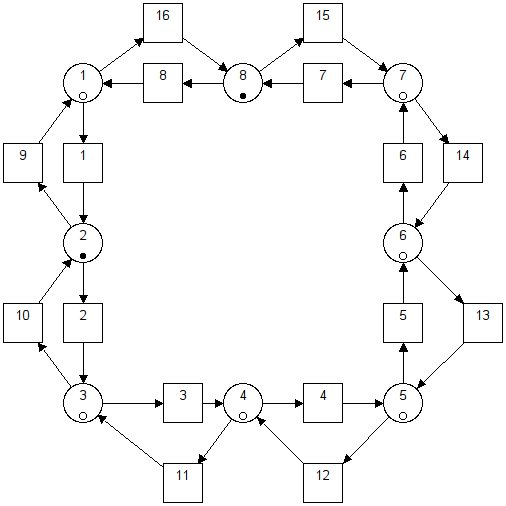
\includegraphics[width=\textwidth]{aufgabe1.png}
        \caption{Simples Gleis}
        \label{img:aufg1}
	\end{figure}
	
	Hier repräsentiert jeder Token einen Zug, die jeweils in beide Richtungen von Gleisabschnitt (Stelle) zu Gleisabschnitt (Stelle) fahren können, sofern in dem betreffenden Abschnitt noch kein Zug voranden ist.
	
\section{Aufgabe 2}
	\subsection{Weiche}	
		\begin{figure}[H]
			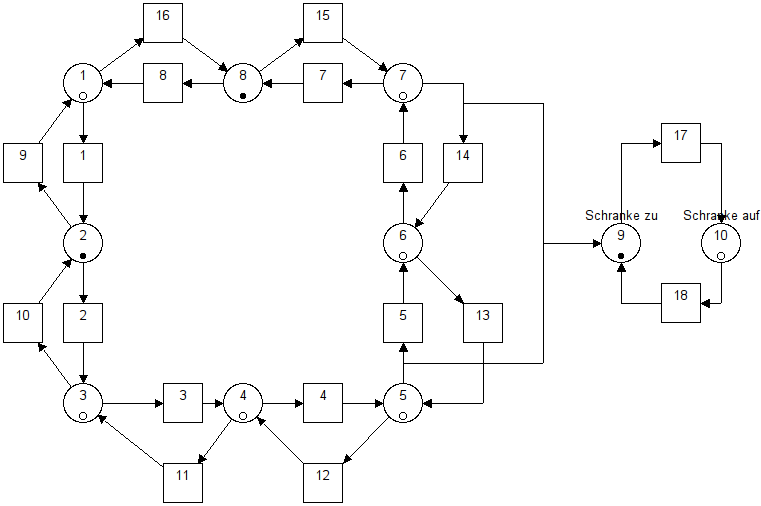
\includegraphics[width=\textwidth]{aufgabe21.png}
        	\caption{Weiche}
        	\label{img:aufg2}
		\end{figure}
	Durch die Schranke wird der Zugang zum Gleisabschnitt 6 kontrolliert. Bei geschlossener Schranke kann ein Zug in diesen einfahren, bei geöffneter Schranke nicht. Die Schranke kann geöffnet werden während sich ein Zug im Gleisabschnitt 6 befindet\footnote{Es ergibt sich für Fussgänger und Autofahrer die Chance einen Darwin Award zu erhalten}.	
		
\end{document}

